
To understand the impact of model evolution in MBT suites, we observed two industrial projects (SAFF and BZC) from industrial partners. Both systems were developed in the context of a cooperation between our research lab and two different companies, Ingenico do Brasil Ltda and Viceri Solution Ltda. The SAFF project is an information system that manages status reports of embedded devices; and BZC is a system for optimizing e-commences logistic activities.  

The projects were run by two different teams. Both teams applied agile practices and used CLARET for use case specification and generation of MBT suites. 

Both projects use manually executed system-level black-box test cases for regression purposes. In this sense, test case historical data is very important since it can help to keep track of the system evolution and to avoid functionality regression. However, the teams reported that often discard test cases when the related steps on the system use cases are updated in any form, which they refer to as a practical management problem.

%We asked the teams to register in a repository all use case updates, as well as all their test suites. Before releasing dates, the teams run all tests to ensure that features already implemented in the software had not been impacted by the recently added ones. Thus, our study 
Therefore, we mined the projects repositories, traced each model change (use case update), and analyzed its impact on the generated suites.

Our goal in this study was to better understand the impact of model updates in the test suites and to measure how much of a test suite is discarded. To guide this investigation, we defined the following research questions:

\begin{itemize}
    \item \textbf{RQ1}: How much of a test suite is discarded due to use case editions?
    \item \textbf{RQ2}: What is the impact of \textit{low}  (syntactic) and \textit{high} (semantic) model edits on a test suite?
    \item \textbf{RQ3}: How much of an obsolete test case needs revision to be reused?
\end{itemize}

\subsection{Study Procedure} 
For each CLARET file (use case model), we collected the history of its evolution in a time frame. In the context of our study, we consider a use case evolution any edit found between two consecutive versions of a CLARET file. Our study worked with 28 use cases, a total of 79 versions, and an average of 5 step edits per CLARET file. Table \ref{tab:useCases} presents the summary of the collected data. After that, we collected the test suites generated for each version of the CLARET files. 
%Both teams used a version control system for managing both code and 

% \begin{table}[]
% \centering
% \caption{Summary of data}
% \label{tab:useCases}
% \begin{tabular}{|l|l|l|l|}
% \hline
%      & \#Use Cases & \#Versions & Mean of Edits \\ \hline
% SAFF &     13      &      42    &     7         \\ \hline
% BZC  &      15     &      37    &     3         \\ \hline
% %  &             &               &               \\ \hline
% \end{tabular}
% \end{table}

\begin{table}[]
\centering
\caption{Summary of the artifacts used in our study.}
\label{tab:useCases}
\begin{tabular}{|l|l|l|l|}
\hline
     & \#Use Cases & \#Versions &\#Edits \\ \hline
SAFF &     13      &      42    &     415         \\ \hline
BZC  &      15     &      37    &     103        \\ \hline
Total  &      28     &      79    &     518         \\ \hline
\end{tabular}
\end{table}

%All suites were generated by using the depth-first-search (DFS) algorithm with one-loop-coverage.

\begin{figure}[h]
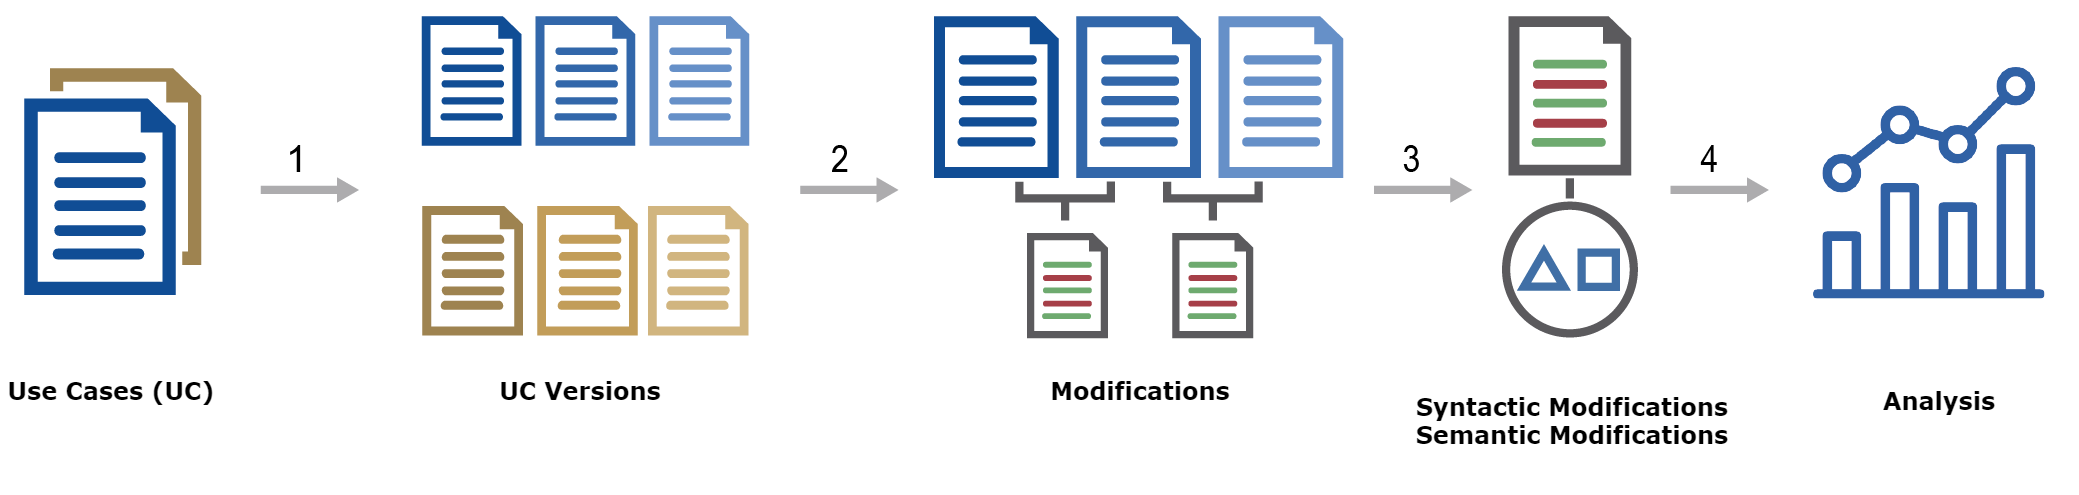
\includegraphics[height=1.2in, width=3.3in]{figs/procedure_flow.png}
\caption{Procedure.}
\label{fig: procedure_flow}
\end{figure}

We extracted a change set for each pair of adjacent versions of a CLARET file (\textit{uc}, \textit{uc'}). 
%This set comprises all changes between \textit{uc} and \textit{uc'}. 
In our analysis, we considered two kinds of edits/changes: i) \textit{step update}. Any step in the base version (\textit{uc}) that had its description edited in the delta version; and ii) \textit{step removal}. Any step that existed in \textit{uc} but not in \textit{uc'}. We did not consider step additions. Since our goal was to investigate reuse in a regression testing scenario, we considered suites generated using only the base version (\textit{uc}). Consequently, no step addition could be part of the generated tests.  

After that, we connected the changeset to the test suites. For that, we ran a script that matched each edited step to the test cases it impacted. We say a test case is impacted by a modification if it includes at least one modified step from the changeset. Thus, our script clustered the tests based on \citet{de2016full}'s classification:
\textit{Obsolete}. Test cases that include updated or removed steps. These tests have different actions or system responses, when compared to its previous version; and \textit{Reusable}. Test cases that exercise only unmodified parts of the model specification. All their actions and responses remained the same when compared to its previous version. Figure \ref{fig: procedure_flow} summarizes our study procedure.

To observe the general impact of the edits, we measured how much of a test suite was discarded due to use case edits. Being $s\_total$ the number of test cases generated from a use case (\textit{uc}); $s\_obs$, the number of found obsolete test cases; and $N$ the number of pairs of use cases; we define the \textit{Average number of Obsolete Test Cases} (AOTC) by Equation \ref{eq:imp}. 

\begin{equation} \label{eq:imp}
AOTC = (\sum \frac{s\_obs}{s\_total}) * \frac{1}{N}
\end{equation}

Then, we manually analyzed each element from the changeset and classified them into \textit{low impact} (syntactic edit), \textit{high impact} (semantic edit), or a combination of both. For this analysis, we defined three versions of the AOTC metric: AOTC\_syn, the average number of obsolete test cases due to low impact edits; AOTC\_sem, the average number of obsolete test cases due to high impact edits; and AOTC\_both, that considers tests with low and highly impacted steps.

Finally, to investigated how much of a test case needs revision, for each test, we measured how many steps were modified. For this analysis, we defined the AMS (Average Modified Steps) metric (Equation \ref{eq:ams}), which measures the proportion of steps that need revision due to model edits. Being $tc\_total$ the number of steps in a given test case; $tc\_c$, number of steps that need revision; and $N$ the number of test cases: 

\begin{equation} \label{eq:ams}
AMS = (\sum \frac{tc\_c}{tc\_total}) * \frac{1}{N}
\end{equation}

\subsection{Results and Discussion}
Our results evidence that MBT test suites can be very sensitive to any model evolution. A great number of test cases were discarded. On average, 86\% (AOTC) of a suite's tests turned obsolete between two consecutive versions of a use case file (Figure \ref{fig: prop_reus_obs}). This result exposes one of the main difficulties of using MBT in agile projects, requirement files are very volatile. Thus, since test cases are derived from these models, any model edit leads to a great impact on the generated tests. 

Although a small number of test cases were reused, the teams in our study found the MBT suites useful. They mentioned that a series of unnoticed faults were detected, and the burden of creating tests was reduced. Thus, we can say that MBT suites are effective, but there is still a need for solutions for reducing test case discard due to model updates.
\\
\\
\noindent
\vspace{2mm} %5mm vertical space
\fbox{\begin{minipage}{23em}
\textbf{RQ1: How much of a test suite is discarded due to use case editions?}
On average, 86\% of the test cases became obsolete between two versions of a use case model.
\end{minipage}}
\vspace{2mm} %5mm vertical space


%Regarding the test cases that became obsolete, 
We manually analyzed each obsolete test case. 
%and classified them as \textit{only low impact}, \textit{only semantic}, or \textit{a combination of both}. 
Figure \ref{fig: prop_obs_by_type} summarizes this analysis. As we can see, 52\% of the cases became obsolete due to \textit{low impact} (syntactic) edits in the use case models, while 21\% were caused by high impact (semantic) changes, and 12\% by both syntactic and semantics changes in the same model. Therefore, more then half of the obsolete set refer to edits that could be easily revised and turned to reusable without much effort (\textit{e.g.}, a step rephrasing, typo fixing). 

\begin{figure}[h]
\centering
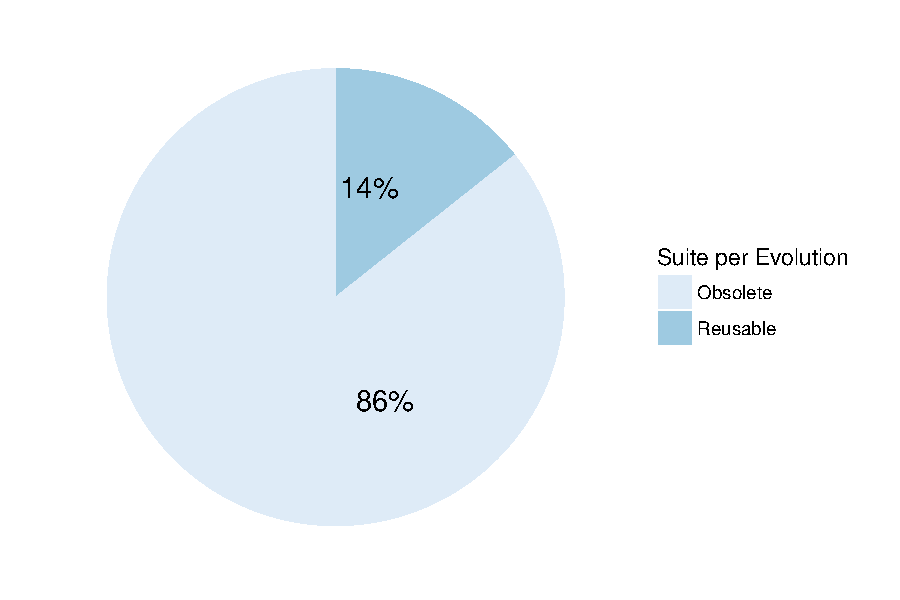
\includegraphics[width=.48\textwidth]{figs/v2_prop_reus_obs.pdf}
%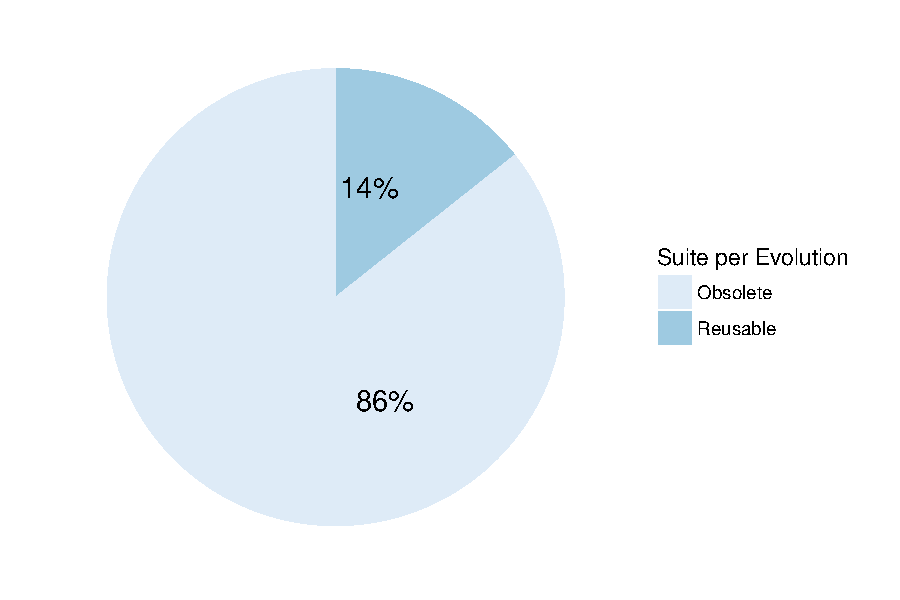
\includegraphics[width=3.3in]{figs/v2_prop_reus_obs.pdf}
\caption{Reusable and obsolete test cases.}
\label{fig: prop_reus_obs}
\end{figure}

\begin{figure}[h]
\centering
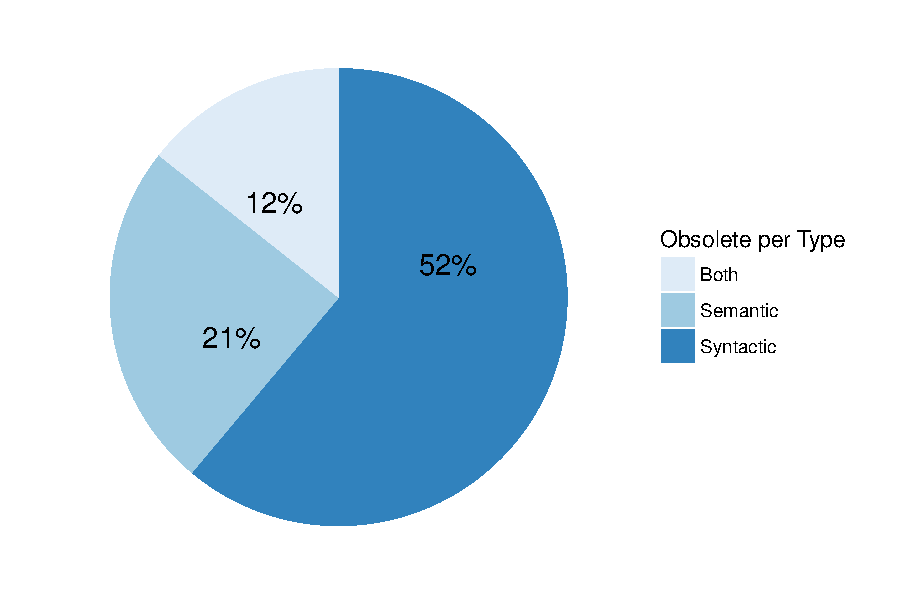
\includegraphics[width=.48\textwidth]{figs/v2_prop_obs_by_type.pdf}
%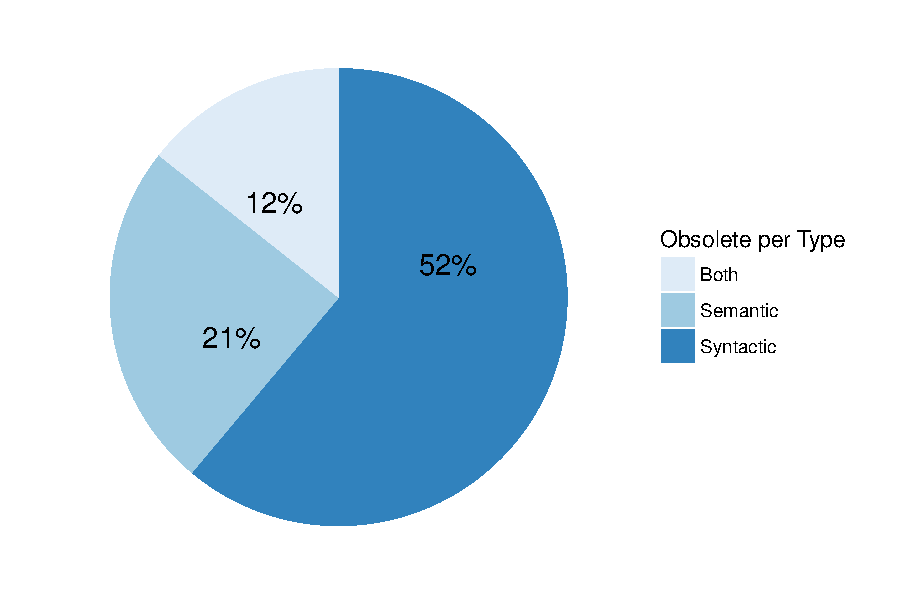
\includegraphics[height=2.3in, width=3.3in]{figs/v2_prop_obs_by_type.pdf}
\caption{Tests that became obsolete due to a given change type.}
\label{fig: prop_obs_by_type}
\end{figure}


\noindent
\fbox{\begin{minipage}{23em}
\textbf{RQ2: What is the impact of \textit{low}  (syntactic) and \textit{high} (semantic) model edits on a test suite?}
52\% of the found obsolete tests were caused by \textit{low impact} use case edits (syntactic changes), while 21\% were due to \textit{high impact} edits (semantic chances), and 12\% by a combination of both.
\end{minipage}}
\vspace{2mm} %5mm vertical space


We also investigated how much of an obsolete test case would need to be revised to avoid discarding. It is important to highlight that this analysis was based only on the number of steps that require revision. We did not measure the complexity of the revision. Figure \ref{fig: prop_tc_steps_impact} shows the distribution of the found results. As we can see, both medians were similar (25\%). Thus, often a tester needs to review 25\% of a test case to turn it reusable, disregarding the impact of the model evolution. 

As most \textit{low impact} test cases relate to basic syntactic step updates (e.g., fixing typos, rephrasing), we believe the costs of revisiting them can be minimal. For the highly impacted tests (semantic changes), it is hard to infer the costs, and, in some cases, discarding those tests can still be a valid option. However, a test case discard can be harmful and should be avoided. 

%However, due to its great impact, the updates needed to turn an obsolete test case due to semantic chances reusable tend to be more complex. Thus, when aiming at improving the number of reusable test cases, a tester should guide efforts on revising the impact of semantic model edits to the test cases.

%50\% of the obsolete test cases by syntactic changes had less than 25\% of their steps impacted. This implies a minimal effort to review these tests to turn them reusable. This demonstrates that aiming at improving the number of reusable test cases, a tester could focus on the semantic model edits since they bring specification changes and functionalities impact.

\begin{figure}[h]
\centering
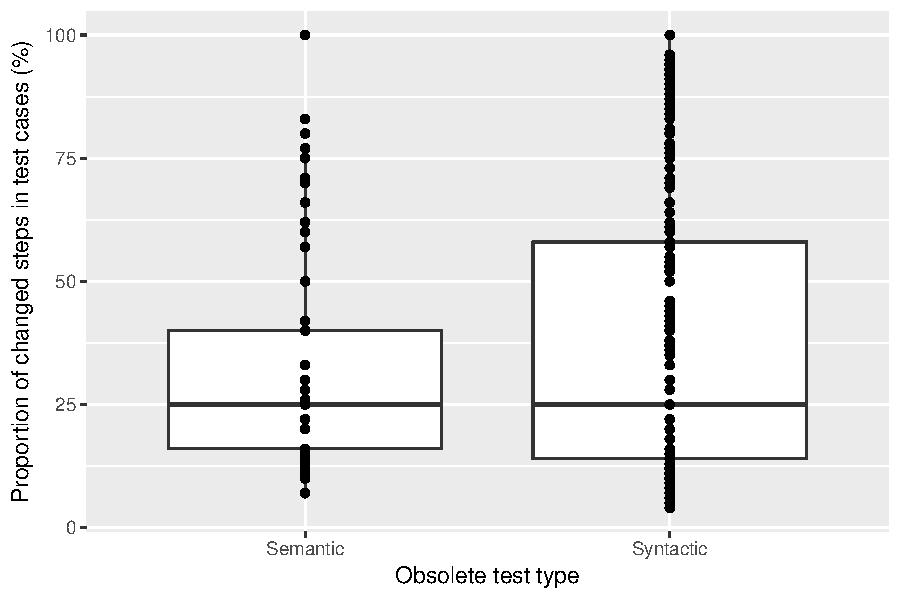
\includegraphics[height=2.5in, width=3.3in]{figs/prop_tc_steps_impact.pdf}
\caption{Proportion of the test cases modified by edit type.}
\label{fig: prop_tc_steps_impact}
\end{figure}

\noindent
\vspace{2mm} %5mm vertical space
\fbox{\begin{minipage}{23em}
\textbf{RQ3: How much of an obsolete test case needs revision to be reused?}
In general, a tester needs to revisit 25\% of the steps of an obsolete test, regardless of the impact of the model edits.
\end{minipage}}
\vspace{2mm} %5mm vertical space

%\subsection{Discussion}% \textcolor{red}{so...?}}
% We can summarize the findings of our study as follows:
% \begin{itemize}
% \item The analyzed MBT suites were highly impacted by use case editions;
% \item In the context of our study, most edits were related to syntactic edits, which can be related to the frequency that use case files are updated in an agile project;
% \item New efforts are needed for improving the use of MBT in agile development. A considerable number of tests were discarded, even though they were being related to only syntactic edits (e.g., sentences rephrasing or typo fixing);
% \item On average, 25\% of the steps of an obsolete test case needed revision in order to turn it reusable. However, the effort for updating a test affected only by syntactic editions seemed to be lower.
% \end{itemize}


% \subsection{Threats to validity}
% Here we list some threats to validity related to our study. Most of them are related to the number of projects or use cases used. Since we worked with industrial artifacts, it was not possible to obtain a broader dataset.

% Regarding external validity, we understand our results cannot be generalized beyond the projects we run our study. However, our study dealt with real industrial artifacts (systems and use case specifications) from different contexts. Therefore, we believe our findings would be similar for projects with similar characteristics (\textit{e.g.}, agile, natural language-based specification, MBT).

% As for conclusion validity, one may argue our study deals with a small sample. Since we worked in the context of our industrial partners, the data available for analysis were limited. However, the artifacts we used were thoroughly validated by the team's engineers and the authors.

% Regarding internal validity,  we applied a manual process for collecting the set of changes and classifying the changes into syntactic or semantic. This process was performed by the first author and later validated by the others. Moreover, the first author had total access to the project's teams for consultation.